\documentclass[twocolumn, unnumberedsubsub]{summery_3.1}
\title{Experimentalphysik III - Zusammenfassung}

\begin{document}
\maketitle
\tableofcontents

\section{Licht}
\subsection{Fermat's Prinzip}
Die geometrische Optik lässt sich mathematisch elegant beschreiben wenn man den Lichtweg 
\(L = \int \abs{\vec r(t)}\cdot n(\vec r (t)) \dt\) definiert. Er ist der normale Weg, gewichtete 
mit dem lokalen Brechungsindex.
Das Licht nimmt immer den Weg, der den Lichtweg extremal werden lässt.
Zur Erinnerung: Es gilt \(n = \frac{c}{v}\)

Es Weg des Lichts kann daher formal mithilfe der Euler-Lagrange Gleichungen beschrieben werden:
\begin{align*}
    \dd {}t \pp{\mathcal L}{\dotv x} = \pp{\mathcal L}{\vec x} \with \mathcal L = \abs{\vec r(t)}\cdot n(\vec r (t))
\end{align*}

\subsection{Snell's Gesetz}
Reist ein Lichtstrahl von einem Medium mit Brechungsindex \(n_1\) in ein zweites mit 
Brechungindex \(n_2\), wird er gebrochen. Der Winkel kann mithilfe von Snell's Gesetz 
berechnet werden:
\begin{align*}
    \frac{\sin\beta}{\sin\alpha} &= \frac{n_a}{n_b}
\end{align*}

\section{Strahlenoptik}
\subsection{Allgemein}\tight
\begin{align*}
    &\te{Abbildungsma{\ss}stab:} & \beta &= \frac BG\\
    &\te{Gegenstandsweite:} & g &\cong \te{Distanz Linse/Gegenstand}\\
    &\te{Bildweite:} & b &\cong\te{Distanz Linse/Bild}\\
    &\te{Gegenstand:} & G &\cong\te{Gegenstand}\\
    &\te{Bild:} & B &\cong\te{Bild}\\
    &\te{Abbildungsma{\ss}stab:} & \beta &= \frac BG\\
    &\te{Deutliche Sehweite:} & s_0 &= 25\,\mathrm{cm}\\
    &\te{Vergrö{\ss}erung:} & V &= \frac{\varepsilon}{\varepsilon_0}\\
    &\te{Numerische Apperatur:} & A_N &= n\sin\alpha\\
\end{align*}

\subsection{Listing'sche Strahlenkonstruktion}
\begin{enumerate}
    \item Haubtstrahl: Trifft auf die Mitte der Linse, die Symmetrie fordert, dass 
    der Strahl bei Linsen gerade durch geht, und bei Spiegeln mit Einfallswinkel gleich Ausfallswinkel
    reflektiert wird. 
    \item Achsenparallele: Geht vom Gegenstand parallel zur optischen Achse. Wird in paraxialer Näherung 
    auf den Brennpunkt gebrochen (Linsen), bzw. zum Brennpunkt hin oder weg gespiegelt (Spiegel).
    \item Brennstrahl: Analog zum Knotenpunktstrahl.
\end{enumerate}
Nie Vergessen den entstehenden Bildpunkt zu kennzeichnen mit \(B\), und von der optischen Achse einen 
orthogonalen Sprich zu \(B\) hochzuziehen, um den gesamten Gegenstand anzudeuten. 
Für mehrere Linsen in einer Reihe, wird erst der (virtuelle) Bildpunkt der ersten Linse konstruiert,
anhand dessen dann der nächste Bildpunkt konstruiert wird.

\subsection{Dünne Linsen in paraxialer Näherung}

\subsubsection*{Linsengleichungen:}\tight
\begin{align*}
    \frac 1g + \frac 1b &= \frac 1f&&\te{und}&
    \frac{b}{g} &= \frac BG   
\end{align*}
Diese Gleichung gilt auch für Spiegel. Achtung: Für einen konvexe Spiegel 
sind zuwohl Bildweite als auch Brennweite negativ!\tight


\subsubsection*{Linsenmachergleichung:}\tight
\begin{align*}
    D = \frac {n_0}f = (n_L - n_0)\hug{\frac 1{r_1} + \frac 1{r_2}}
\end{align*}\ttight

\subsubsection*{Brechkraft eines optischen Systems:}\tight
\begin{align*}
    D &= D_1 + D_2 - d D_1 D_2\with d\cong \te{Distanz zwischen Linsen}
\end{align*}

\subsection{Dicke Linsen}
\subsubsection*{Linsenmachergleichung:}\tight
\begin{align*}
    D = \frac {n_0}f &= (n_L - n_0)\hug{\frac 1{r_1} + \frac 1{r_2}}
    + \frac{(n_L - n_0)^2}{n_L}\frac{d}{r_1r_2}
\end{align*}\ttight

\subsubsection*{Haubtebenen:}
\tight
\begin{align*}
    h_1 &= \frac{n_L - n_0}{n_L} \frac{f d}{r_2}\\
    h_2 &= -\frac{n_L - n_0}{n_L} \frac{f d}{r_1}
\end{align*}\ttight

\subsubsection*{Newtonsch'sche Abbildungsgleichung}\tight
\begin{align*}
    z\cdot z' &= f_B \cdot f_G
\end{align*}\ttight


\subsection{Matrizen-Optik}
Sind vom Gegenstandspunkt aus gesehen, die vom Licht durchlaufenden Strecken \(s_1,s_2,\dots,s_n\),
so ist die korrekte Matrix gegeben durch \(M_n\cdot {\dots} \cdot M_2\cdot M_1\). Die Matrizen müssen somit 
anderrum multipliziert werden.
Ein optisches Gerät ist dann scharf eingestellt wenn \(M\cdot (\alpha,0)^T = (\beta,0)^T\).
\begin{align*}
    &\te{Zustandsvektor:} & \vec v &= \binom{x}{n\alpha}\\
    &\te{Freie Ausbreitung:} & \mat M_T &= \begin{pmatrix}
        1 & \frac{s}{n_0}\\
        0& 1
    \end{pmatrix}\\
    &\te{Brechung:} & \mat M_B &= \begin{pmatrix}
        1 & 0\\
        \frac{n_0-n_L}{R} & 1
    \end{pmatrix}\\
    &\te{Dünne Linse:} & \mat M_L &= \begin{pmatrix}
        1 & 0\\
        -D & 1
    \end{pmatrix}\\
    &\te{Dicke Linse:}
\end{align*}\tight
\begin{align*}
    \mat M_{\bar L} &= \begin{pmatrix}
        1-\frac{n_L-n_0}{n_L}\frac{d}{R_1} & \frac{d}{n_L}\\
        -D & 1+\frac{n_L-n_0}{n_L}\frac{d}{R_2}
    \end{pmatrix}
\end{align*}
 
\subsection{Bildfehler}
\begin{figure}[H]
    \centering
    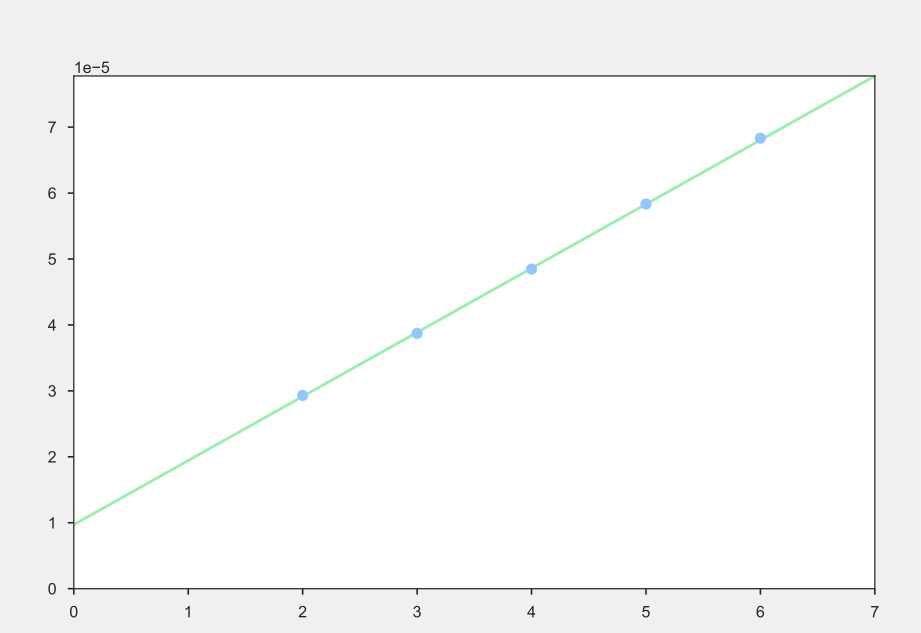
\includegraphics[width=0.4\textwidth]{3.png}
\end{figure}
\subsubsection*{A. Koma:}
Parallele Lichtstrahlen fallen in einem Winkel auf die Linse. Ist die überlagerung zweier anderer Bildfehler,
dem Astigmatismus und der Sphärischen Abberation.\tight

\subsubsection*{B. Sphärische Abberation/Öffnungsfehler:}
Dieser Bildfehler entsteht dadurch, dass die Kugel nicht die mathematisch perfekte Form 
ist um parallele Lichtbündel auf einen Punkt zu fokossieren; dies währe ein Paraboloid.
Die Kugel ist achsenfern stärker gekrümmt als die Parabollinse, und hat daher dort eine 
stärkere Brechkraft. Der Fokuspunkt von achsenfernen Licht liegt folglich näher an der Linse. \tight

\subsubsection*{C. Chromatische Abberation:}
6Die Ursache der chromatischen Abberation ist, dass die Brechkraft der Linse eine Funktion der Wellenlänge des 
Lichts ist. Folglich werden verschiedene Wellenlängen auf verschiedene Brennpunkte fokossiert. 
Ein Linsensystem das keine chromatische Abberation aufzeigt (zumindest in erster Ordung), 
also \(\pp f\lambda=0 \implies \pp{f}{n(\lambda)} =0\), nennt sich Achromat.\tight

\subsubsection*{D. Verzeichung:}
Verzeichnung ist ein Lagefehler und bedeutet, dass die Bildhöhe (Abstand eines Bildpunktes vom Bildzentrum)
auf nichtlineare Weise von der Höhe des entsprechenden Objektpunktes abhängt. Man kann auch sagen: Der Abbildungsmaßstab hängt von
der Höhe des Objektpunktes ab.h Es können sowohl kissenförmige als auch tonnenförmige Verzeichungen entstehten.\tight

\subsubsection*{E. Astigmatismus:}
Astigmatismus tritt bei "schiefen Strahlen"{} auf. die Ursache ist, dass das 
Strahlenbündel entlang der Maridional- und der Sagittalebene unterschiedlich stark gebrochen wird.

\subsection{Vergrößerung}
    Winkelvergrößerung allgemein:
\begin{align*}
    V &= \frac{\te{Winkel mit Instrument}}{\te{Winkel ohne Instrument}}=\frac{\varepsilon}{\varepsilon_0}
\end{align*}
    \emph{Lupe}:
\begin{align*}
    V &= \frac{s_0}{f}
\end{align*}
    \emph{Mikroskop}, Abbildungsmaßstab des Objektives, Okularvergrößerung:
\begin{align*}
    \Gamma_{ob}&\approx \frac t{f_{ob}} \with t\hat=\te{Tubuslänge} \\
    V&= \Gamma_{ob} V_{ok} =\frac{ts_0}{f_{ob}f_{ok}} 
\end{align*}
    \emph{Teleskop}:
\begin{align*}
    V&= \frac{f_{ob}}{f_{ok}}
\end{align*}


\section{Fotometrie}
\subsection{Allgemein}
\begin{figure}[H]
    \centering
    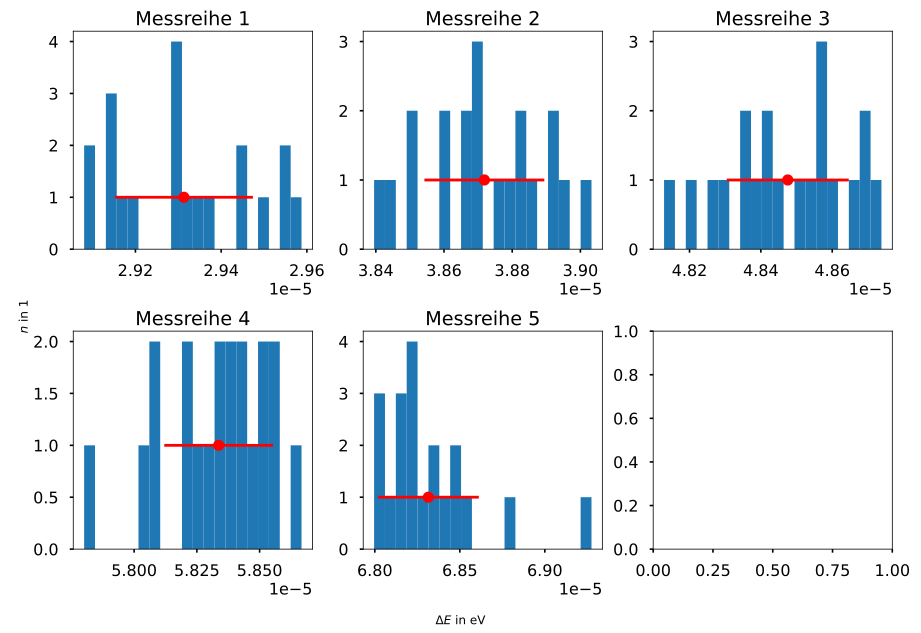
\includegraphics[width=.5\textwidth]{1.png}
\end{figure}

\subsection{Gesetze}
\subsubsection{Stefan-Boltzmann-Gesetz:}\tight
    \begin{align*}
        \Phi_E &= \sigma \cdot A \cdot T^4\\
        \sigma &= 5.670 \cdot10^{-8} \ufrac{W}{m^2K^4}\note[Stefan-Boltzmann-Konstante]
    \end{align*}\ttight

\subsubsection{Wien'sches Verschiebungsgesetz:}
    Ist \(\lambda_{\te{max}}\) die Wellenlänge, bei der die Emission eines Schwarzerkörpers
    die maximale Intensität zeigt, so gilt:
    \begin{align*}
        \lambda_{max}\cdot T = \const = 2.8978 \E{-3} \mathrm{m\, K}
    \end{align*}\ttight

\subsubsection{Rayleigh-Jean-Gesetz:}
    Das Rayleigh-Jean-Gesetz beschreibt die Abstrahlungsleistungspektrum bei hohen Wellenlängen:
    \begin{align*}
        M_E(\lambda):= \frac{\mathrm  d \Phi_E(\lambda)}{\mathrm d\lambda}=2\pi k c\frac T{\lambda^4}
    \end{align*}\ttight

\subsubsection{Wien'sches Strahlungsgesetz:}
    Das Wien-Gesetz beschreibt die Abstrahlungsleistungspektrum bei niedrigen Wellenlängen:
    \begin{align*}
        M_E(\lambda) &= \frac{c_1}{\lambda^5} \frac{1}{e^{\frac{c_2}{\lambda T}}}
        = \frac{2\pi h  c^2}{\lambda^5} \frac{1}{e^{\frac{h c}{k_B}\frac{1}{\lambda T}}}
    \end{align*}\tight

\section{Wellenoptik}
\subsection{EM-Wellen:}
Eine ebene Welle wird mathematisch beschrieben durch:
\begin{align*}
    \mat E = \mat E_{0} e^{i(\omega t - \mat k \cdot \mat r)}\note \mat E_0\in\C^3, \mat k \in \R^3
\end{align*}
Ist \(\mat E_0\cdot \mat k = 0\), so schwingt die Welle nicht in Richtung ihrer Ausbreitungsrichtung und
ist somit als eine Longitudinal-Welle zu identifizieren. Dies ist für EM-Wellen im Vakuum der Fall.
Ist der Phasendifferenz zwischen den beiden Komponenten in \(\mat E_0\) die orthogonal zur 
Bewegungsrichtung sind gleich null, so schwingen E-/ und B-Feld in Phase, die Welle ist 
\emph{linear polarisiert}. Für \(\Delta \phi = \frac\pi2\) ist die Norm des Feldes zeitlich konstant, 
der Feldvektor rotiert nur um die Bewegungsrichtung; dieser Fall nennt sich \emph{zirkulare Polarisation}.
Liegt der Winkel hingegen irgendwo dazwischen, so rotiert der Feldvektor auf elliptischen 
Bahnen, daher der Name \emph{elliptische Polarisation}.


Überlagern sich die Amplituden zweier kohärenter Wellen, so ist die 
Intensität:
\begin{align*}
    \tug I &= 4 \tug{I_0} \cos^2 \hug{\frac{\Delta \phi}{2}}
\end{align*}
 
Und allgemein für zwei Wellen mit Phasendifferenz \(\Delta\phi\):
\begin{align*}
    \tug{I} &= \varepsilon_0 c \tug[\big]{(\v E_1 + \v E_2)^2}\\
    &= \varepsilon_0 c \bug{\tug[\big]{\v E_1^2} + 2\tug[\big]{\v E_1 \v E_2} + \tug[\big]{\v E_12^2}}\\
    &= \tug[\big]{I_1} + \tug[\big]{I_{12}} + \tug[\big]{I_2}\\
    \tug{I_{12}} &= \varepsilon_0 c E_{01} E_{02} \cos(\Delta \phi)
    = \varepsilon_0 c \sqrt{\tug{I_1}\tug{I_2}} \cos(\Delta \phi)
\end{align*}

\subsection{Kohärenz}
\subsubsection*{Zeitliche Kohärenz}
Zeitspanne \(\Delta t_c\) in der sich die Phasendifferenz 
\(\Delta\phi_{12}(\v r, t) = \phi_1(\v r, t) - \phi _2(\v r, t)\) um weniger als
\(2\pi\) ändert. 
\begin{align*}
    \Delta t \Delta f \approx 1
\end{align*}

Man definiert hier auch die Kohärenzlänge \(\Delta l_c= c\cdot \Delta t_c\).

\subsubsection*{Räumliche Kohärenz}
Analog definiert man die räumlihe Kohärenz, wenn eine Wellenfront ihre Phasendifferenz
\(\Delta\phi_{12}(\v r, t) = \phi_1(\v r, t) - \phi _2(\v r, t)\) zwischen zwei 
an zwei Orten um weniger als \(2\pi\) ändert.

\subsubsection*{Kohärenzlänge realer Lichtquellen}
Die Emission eine Wellenzuges durch ein angeregtes Atom dauert ca. 1 bis 10ns 
(\(=\Delta t_c\)). In einem Wellenzug koexistieren verschiedene Frequenzen, die einer 
Verteilung folgen. Man nennt \(\Delta f = \frac 1{\Delta t_c}\) die Frequenzbreite.
Die Kohärenzlänge lasst sich in erster Näherung berechnen als 
\(l_c = \frac{\lambda^2}{\Delta \lambda}\).

\subsection{Interferenzphänomene}
\subsubsection{Doppenspalt:}\tight
\begin{align*}
    &\te{Maxima:} & \sin\theta_{max} &= \frac{n\lambda}{d}\\    
    &\te{Minima:} & \sin\theta_{min} &= \hug{n+\frac12}\frac{\lambda}{d}  
\end{align*}\tight

\subsubsection{Einzelspalt:}\tight
\begin{align*}
    &\te{Maxima:} & \sin\theta_{max} &=  \hug{n+\frac12}\frac{\lambda}{d}\\    
    &\te{Minima:} & \sin\theta_{min} &= \frac{n\lambda}{d}    
\end{align*}\tight

\subsubsection{Gitter:}
\(N\)-Spalte mit Abstand \(g\).
\begin{align*}
    &\te{Maxima:} & \sin\theta_{max} &=  \frac{n\lambda}{g}\\    
    &\te{Minima:} & \sin\theta_{min} &= \hug{n+\frac1N}\frac{\lambda}{g}    
\end{align*}\tight

\subsubsection{Maximale Ordnung:}
Es gibt eine maximale Ordnung, denn der Winkel muss kleiner \(90^\circ\) sein \(1\ge\sin\alpha\). Für den Doppelspalt/Gitter würde sich 
\(n_{\te{max}}\le\frac d\lambda\) ergeben.

\subsubsection{Überlappung von Spektren}
Die Spektren zweier benachbarter Ordnungen überlappen sich, wenn 
\(\theta_{\te{max}}(\lambda_{\te{max}}, n) > \theta_{\te{max}}(\lambda_{\te{min}}, n+1)\) gilt.
Für Doppelspalt und Gitter ergibt sich damit, Überlappung für:
\begin{align*}
    n > \frac{\lambda_{\te{min}}}{\lambda_{\te{max}} - \lambda_{\te{min}}}
\end{align*}

\subsubsection{Auflösungsvermögen/Rayleighkriterium:}
Zwei Wellenlängen \(\lambda\) und \(\lambda + \Delta \lambda\) können getrennt werden, sobald das Maximum 
zu \(\lambda + \Delta \lambda\) im ersten benachbarten Minimum liegt.
Für ein Gitter ergibt sich damit: \(\frac{\lambda}{\Delta \lambda} = n N\).

\subsection{Beugungsphänomene}
\subsubsection*{Frauenhofer Beugung:}
Abstand des Objektes zum Schirm  gro{\ss} \(\to\) Stahlen annähernd parallel
\(\to\) Beugungsbild nur Richtungsabhängig.

\subsubsection{Fresnel Beugung:}
Abstand des Objektes zum Schirm \emph{nicht} gro{\ss} \(\to\) 
Stahlen nicht parallel \(\to\) Beugungsbild Distanz und Richtungsabhängig.

\subsubsection{Fresnel-Kirchhoff'sches Beugungsintegral}
Die Amplitude und Phase auf einem Schirm \((z=0)\) sei durch \(\vec E_0(x,y)\) 
und \(\phi(x,y)\) gegeben. Dann ist die Amplitude an einem
Punkt $P=(x,y,z)^T$:
\begin{align*}
    \vec E_P(x,y,z) &= \iint\limits_{z=0} K(\beta)\frac{\vec E_0(x',y')}{r_A} 
    e^{i(\phi(x',y') - k r_A)} \dx'\dy'\\
    \te{mit } r_A &= \sqrt{(x-x')^2 + (y-y')^2 + z^2}
\end{align*}

\subsubsection{Fresnel-Linse}\tight
\begin{align*}
        &\te{Radien:}  & r_n &= 
        \sqrt{n\lambda f + \frac{n^2\lambda^2}4} \overset{f\gg n\lambda}{\approx} \sqrt{n\lambda f}
\end{align*}

\subsubsection{Lochblende}
Position der ersten Minima und Maxima hinter einer Lochblende. 
Angegeben sind die Werte für $\frac{k D}{2\pi} \sin \theta_{min}$ bzw. 
$\frac{k D}{2\pi} \sin \theta_{max}$. 
Au{\ss}erdem ist die Intensität der Nebenmaxima im Verhältnis zum zentralen
Maximum angegeben.
\begin{figure}[H]
    \centering
    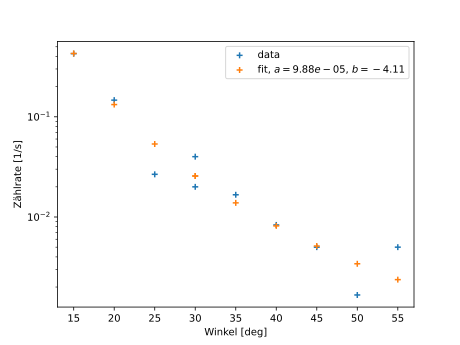
\includegraphics[width=0.5\textwidth]{2.png}
\end{figure}

\subsubsection{Rayleigh-Kriterium}
Die maximale Auflösung eines optischen Systems ist durch Beugungseffekte am 
Rand der Linse fundamental beschränkt. 
Das Rayleigh-Kriterium definiert die minimale auflösbare Winkeldistanz
als die Winkeldistanz bei der 
sich das Beugungsminimum erster Ordnung, des einen Objektes, mit dem
Beugungsmaximum erster Ordnung, des anderen Objektes, überlappen würde. 
Für eine Lochblende gilt:
\begin{align*}
    \sin\theta_{min} =  1.22 \frac{\lambda}{D}
    \ \ \implies \ \ r_{min} =  1.22 \frac{f \lambda}{D}
\end{align*}

\subsubsection{Babinet'sche Prinzip}
Das Babinet'sche Prinzip besagt, dass die Beugungsbilder zueinander komplementärer
Blenden außerhalb des Bereiches, der durch die geometrische Abbildung be-
leuchtet wird gleich ist.

\section{Polarisation}
\subsubsection{Allgemein}
\begin{enumerate}
    \item Lineare Polarisation:\\
    Ein Strahl, dessen \(\vec E\)-Feld in nur einer konstanten Ebene schwingt, z.B 
    $\vec E(\vec r) = \hat E e^{i(\vec k \vec r + \omega t)}$. Er kann als Superposition zweier zirkular polarisierter Strahlen dargestellt werden, 
    die konträren Drehsinn haben.
    \item Zirkulare Polarisation:\\
    Ein Strahl, dessen \(\vec E\)-Feld im Betrag konstant ist, und um die Ausbreitungsrichtung
    kreist. Er kann als Überlagerung zweier orthogonaler, linear polarisierter
    Strahlen dargestellt werden, die zueinnander um \(90^\circ\) phasenverschoben sind.
    \item Optische Achse (Kristalloptik):\\
    Die optische Achse ist bei einem anisotropen Kristall jene Achse, entlang derer 
    jede Polarisationsrichtung den gleichen Brechungsindex hat.
    \item Haubtschnitt:\\
    Der Haubtschnitt ist jene Ebene, die durch die optische Achse und die Ausbreitungsrichtung 
    des Lichts aufgespannt wird.
    \item (Au{\ss}er)Ordentlicher Strahl:\\
    Der ordentliche Strahl eines Lichtstrahls ist jeder Teil dessen \(\vec E\)-Feld \emph{senkrecht}
    zum Haubtschnitt schwingt. Beim au{\ss}erordentlichen findet die Schwingung dem entsprechend 
    in der Ebene (Haubtschnitt) statt.\\
    Die Brechungsindizes von ordentlichem und au{\ss}erordentlichem Strahl sind 
    jeweils \(n_o\) und \(n_{ao}\).
\end{enumerate}

\subsubsection{Polarisationsfilter (Gesetz von Malus)}
\begin{align*}
    I' &= I \cdot \cos^2(\Delta \theta)
\end{align*}

\subsubsection{Lambda/4-Plättchen}
\begin{align*}
\Delta \phi &=\frac{2\pi}{\lambda} d \,\Delta n
\end{align*}

\subsubsection{Fresnel'sche Formeln}
Trifft ein Lichtstrahl unter einem Winkel \(\alpha\) zum Lot auf eine Grenzfläche 
zweier Medien mit Brechungszahlen $n_1$ und $n_2$, so wird er in
einen reflektierten und einen gebrochenen Strahl aufgespalten. Ihre
Amplituden sind durch die Reflexions- und Transmissionskoeffizienten 
für die Anteile an Polarisation in der Einfallsebene (Index p) und
senkrecht dazu (Index n) gegeben:
\begin{align*}
    r_n &= \frac{n_1\cos\alpha - n_2\cos\beta}{n_1\cos\alpha + n_2\cos\beta}\\
    r_p &= \frac{n_2\cos\alpha - n_1\cos\beta}{n_2\cos\alpha + n_1\cos\beta}\\
    t_n &= \frac{2 n_1 \cos\alpha}{n_1\cos\alpha + n_2\cos\beta}\\
    t_p &= \frac{2 n_2 \cos\alpha}{n_2\cos\alpha + n_1\cos\beta}\\
\end{align*}

\subsubsection{Anisotropie durch Spannung}
Setzt man ein Material unter Spannung (Kraftvektor \(\v F\)), kann das Material 
anisotrop werden. Der ordentliche Strahl ist orthogonal zu \(\v F\), der
außerordentliche parallel.

\subsubsection{Faraway Effekt}
Linear polarisiertes Licht wird reist durch ein Material, das von einerm starken 
B-Feld entlang der Ausbreitungsrichtung durchsetzt ist. Es wird dabei 
um einen Winkel \(\alpha = V\, L \, B, \ V=\te{Verdet-Konstante}\) gedreht. Es lässt sich erklären, wenn man das linear polarisierte Licht als 
Überlagerung zweier zirkular polarisierter Strahlen betrachtet. 
Die beiden Wellen regen Elektronen zu einer Kreisbahn an, die einen Dipolmoment erzeugt,
der je nach Richtung energetisch günstig oder ungünstig im B-Feld liegt.

\subsubsection{Kerr-Effekt}
Equivalent zum Faraway Effekt, jedoch wird hier ein E-Feld angelegt. Es bildet sich erneut
ein anisotropes Material, da das äußere E-Feld die Schwingungseigenschaften der Elektronen 
beeinflusst. Die optische Achse liegt entlang der E-Feld Richtung.
Die Erzeugung von Dipolen ist proportional zu \(E\), und die Ausrichtung der 
Dipole auch, insgesamt also \(\propto E^2\):
\begin{align*}
    \Delta n &= n_{ao} - n_o = K \lambda E^2\note K=\te{Kerr-Konstante}\\
    \Delta \phi &= 2\pi L K E^2
\end{align*}

\subsubsection{Pockels-Effekt}
Wie Kerr-Effekt, jedoch linear in \(E\). Der Effekt ist um mindestens eine 
Größenordnung stärker als der Kerr-Effekt, bei gleicher Feldstärke.
Der Effekt ist stark Richtungsabhängig.
\begin{align*}
    \Delta n &= n_{ao} - n_o = n^3 r_{\te{eff}} E \\
    r_{\te{eff}} &= \te{effektiver elektrischer Tensor}
\end{align*}

\subsubsection{Spiegel-Isomerie}
Eine Lösung mit chiralen Molekülen dreht den Winkel des einfallenden linear polarisierten
Licht. 
\begin{align*}
    \alpha &= [\alpha]^T_\lambda \cdot \beta \cdot L \\
    [\alpha]^T_\lambda &= \te{spezifischer Drehwinkekl}\\
    \beta &= \te{Konzentration}\\ 
\end{align*}

\section{Quantenphysik}
\subsection{De-Broglie-Wellenlänge}\tight
\begin{align*}
    \v p &= \hbar \cdot \v k \rightarrow
    p = \hbar \cdot k = \frac{h c}{\lambda}
\end{align*}

\subsection{Planksche Strahlungsformel / Schwarzkörperstrahlung}
\begin{align*}
    P(\nu) &= \frac{h \nu^3}{c^2} \frac{1}{\exp\hug{-\frac{h\nu}{kT}}-1}
\end{align*}

\subsection{Compton-Effekt}
\begin{align*}
    \Delta \lambda &= \frac{h}{m_0c} (1-\cos\theta)  = \lambda_c (1-\cos\theta)
\end{align*}


\subsection{Wellenfunktion}
In der Quantenphysik dreht sich alles um die Wellenfunktion \(\psi/\Psi\), denn sie trägt alle existierenden Informationen 
über ein System gleichzeitig in sich.  
Beobachtbare Größen werden durch lineare, hermitische Operatoren beschrieben, welche auf die Wellenfunktion
wirken können.
Die Eigenvektoren eines solchen  \(\hat A \ket {A_n} = A_n\ket{A_n} \) formen eine 
vollständige, orthonormale Basis. Hat man sich eine passende Basis ausgesucht, 
kann die Wellenfunktion dieser entwickelt werden als 
\(\ket \psi = \sum_n \ket{E_n} \braket{E_n}\psi \).
Die Koeffizienten vor jedem Basisvektor, haben nach der Born-Regel eine wichtige physikalische Bedeutung:
Ihr Norm-Quadrat entspricht der Wahrscheinlichkeit, dass bei einer Messung der dem Basisvektor 
zugehörige Eigenwert gemessen wird.

\subsubsection{Schrödinger Gleichung}
Die Schrödinger Gleichung definiert dem Hamiltonoperator in Orts-Koordinaten, und kann daher verwendet werden,
um die Wellenfunktion eines Systems zu finden.

Zeitunabhängig:
\begin{align*}
        \hat H\ket \Psi&= 
        -\frac{\hbar ^2}{2m} \Delta \ket\psi + V \ket\psi
        =E\ket\psi
\end{align*}
mit \begin{align*}
    \ket{\Psi(t)} = \sum_{n} A_n e^{ {-iE_n t}/\hbar} \ket{\psi_{E_n}}
\end{align*}

Zeitabhängig:
\begin{align*}
    \hat H\ket \Psi &= i\hbar \pp{}t\ket\Psi
\end{align*}

Eine physikalische Wellenfunktion \(\psi\) ist normierbar. Für ein Potenzial \(V(x)=\propto \delta(x)\)
ist die Wellenfunktion in Orts-Basis stetig, für eine unstetiges Potenzial sie stetig diffbar, und 
für ein stetiges Potenzial zweimal diffbar.

\subsection{Operatoren}
\subsubsection{Bra}
Der Bra \(\bra \phi\) wirkt auf einen Vektor \(\ket\psi\) wie ein hermitisches Skalarprodukt
mit dem Vektor \(\ket \phi\):
\begin{align*}
    \bra \phi\ket \psi &= \braket \phi\psi = \int \overline{\phi(x)}\,\psi(x)\dx
\end{align*}

\subsubsection{Hermitisches Konjugat}
Das hermitische Konjugat \(A^\dagger\) eines Operators \(\hat A\), ist definiert als:
\begin{align*}
    \sbraket\psi{\hat A\psi} &= \sbraket{\hat A^\dagger\psi}{\psi}
\end{align*}
Ist der Operator eine Matrix, berechnet sich das hermitische Konjugat als \(\hat M^\dagger = \overline{\hat M ^T}\).
Gilt für einen Operator, dass \(\hat A = \hat A^\dagger\), so nennt man in hermitisch.  

\subsubsection{Unitäre Operatoren}
Ein Operator ist zudem unitär, wenn die Tranformation das Skalarprodukt erhält.
\begin{align*}
    \braket\phi\psi &\peq \sbraket{\hat U \phi}{ \hat U \psi}
    = \sbraket{\phi}{\hat U^\dagger \hat U \psi}\\
    \implies \hat U^\dagger \hat U &= \I
\end{align*}
\begin{align*}
    \rot \v B &= \j + \pp{\v E}t
\end{align*}
\subsubsection{Kommutator}
Der Kommutator ist definiert als:
\begin{align*}
    \scom AB &= \hat A \hat B - \hat B \hat A
\end{align*}
Man sagt, dass zwei Operatoren miteinander kommutieren, wenn \(\scom AB = 0\).  


\subsubsection{Erwartungswert}
Der Erwartungswert \(\tug A\) eines Operators \(\hat A\) errechnet sich als:
\begin{align*}
    \tug A = \sopbraket\psi {\hat A}
\end{align*}

\subsubsection{Standartabweichung}
Für nicht kommutierende Operatoren \(\hat A\) und \(\hat B\) ist die Standardabweichung \(\Delta A,\Delta B\)
gegeben durch:
\begin{align*}
    (\Delta A)^2 &= \sbraket{\psi}{(\hat A - \tug A)^2\psi}
    = \tug {A^2}- \tug A^2\\
\end{align*}

\subsubsection{Wichtige Operatoren}
\begin{enumerate}
    \item Die Identität \(\I\):
    \begin{align*}
        \I &= \sum_i \ket i \bra i 
    \end{align*}
    
    \item Zeitevolution-Operator \(\hat T\) (für zeitinvarianten Hamiltonoperator, und Hamilton-Basis):
    \begin{align*}
        \hat T &= e^{\frac{\hat H t}{i \hbar}} = e^{-i\hat H t/\hbar}\\
        \ket{\psi(t)} &= \hat T \ket {\psi(0)}\\
        &= \sum_n \ket {E_n} \braket {{E_n}}\psi e^{-i E_n t/\hbar}\\
        &= \sum_n \ket {E_n} \braket {E_n}\psi e^{-i \omega t} 
    \end{align*}
    
    \item Impuls-Operator \(\hat p\):
    \begin{align*}
        \hat p &= -i\hbar \nabla \note[Herleitung mit ] \psi(x) = \int\dk e^{i k x}
    \end{align*}
    
    \item Zeitunabhängiger Hamilton-Operator \(\hat E/\hat H\):
    \begin{align*}
        \hat H = \frac{\hat p^2}{2m} + V(x)
        = -\frac{\hbar^2}{2m} \Delta + V(x)
    \end{align*}
    
    \item Drehimpuls-Operator \(\hat L_i\):
    \begin{align*}
        \hat {\vec L} &= \hat {\vec x} \times  \hat {\vec p} \tand
        \hat L_i = \levicivita\, \hat x_j  \hat p_k
    \end{align*}
    Der Operator gehorcht der Drehimpuls-Algebra:
    \begin{align*}
        \scom{L_i}{L_j} &= \levicivita \,i\hbar\, \hat L_k
    \end{align*}
    
    \item Spin-Operator \(\hat S_i\):
    \begin{align*}
        \hat S_i &= \frac\hbar2 \sigma_i\\
        \scom{S_i}{S_j} &= \levicivita  \,i\hbar\,  \hat S_k
    \end{align*}
    mit den Paulimatizen \(\sigma_i\), welche den vierdimensionalen Raum der 
    hermitischen \(2\!\times\!2\)\(\,\)-\(\,\)Matrizen aufspannt.
    \begin{align*}
    \sigma_{0} &= \begin{pmatrix}1&0\\0&1\end{pmatrix}&
    \sigma_{1,x} &= \begin{pmatrix}0&1\\1&0\end{pmatrix}\\
    \sigma_{2,y} &= \begin{pmatrix}0&-i\\i&0\end{pmatrix}&
    \sigma_{3,z} &= \begin{pmatrix}1&0\\0&-1\end{pmatrix}
    \end{align*}
    Für sie gelten folgende nützliche Identitäten:
    \begin{align*}
        \sigma_0^2 &= \sigma_1^2  
        = \sigma_2^2 = \sigma_3^2 = -i\,\sigma_0\sigma_1\sigma_2\sigma_3
    \end{align*}
    \begin{align*}
        \sigma_i &= \sigma_i \inv \tand \com{\sigma_i}{\sigma_j} = \levicivita \,2i\, \sigma_k
    \end{align*}
\end{enumerate}


\subsection{Unschärfenrelationen}
Die Unschärfenbeziehungen lassen sich alsgemein aus 
\begin{align*}
    \Delta A \cdot \Delta B &\ge \frac12 \sabs{\tug[]{\scom AB}}
\end{align*}
herleiten.
\begin{align*}
    \Delta x_i \Delta x_j &\ge 0\\
    \Delta p_i \Delta p_j &\ge 0\\
    \\
    \Delta p_i \Delta x_j& \ge \frac \hbar 2 \delta_{ij}\\
    \\
    \Delta \absv L \Delta L_i &\ge 0\\
    \Delta L_i \Delta L_j &> 0\note i\neq j\\
    \\
    \Delta E \Delta t \ge \frac \hbar 2\\
\end{align*}

\subsection{Zeit-Evolution von Erwartungswerten}
Die zeitliche Evolution des Erwartungswertes eines Operators \(\hat A\)
ist gegeben durch das Ehrenfest-Theorem:
\begin{align*}
    \dd{}t \stug {\hat A} &= \frac 1{i\hbar} \tug[]{\scom AH} + \tug[]{\p_t \hat A}
\end{align*}
Die Herleitung ist recht einfach, an einer Stelle wird die Schrödingergleichung verwendet \(\p_t \ket\psi = \frac1{i\hbar}\hat H \ket\psi\):
\begin{align*}
    \dd{}t \sopbraket \psi{\hat A} 
    &= \hug{\p_t \bra\psi}\hat A \ket \psi
    + \bra\psi\hat A \hug[]{\p_t\ket \psi}
    + \bra\psi \hug[]{\p_t \hat A} \ket \psi\\
    &= \frac{1}{i\hbar}\hug{
        -\hat H\bra\psi\hat A\ket\psi+ 
        \bra\psi\hat A \hat H \ket \psi}
    + \tug[]{\p_t \hat A}\\
    &= \frac{1}{i\hbar}\hug{- \bra\psi\hat H\hat A\ket\psi + \bra\psi\hat A \hat H \ket \psi} + \tug[]{\p_t \hat A}\\
    &= \frac{1}{i\hbar}\tug[]{\scom AH} + \tug[]{\p_t \hat A}
\end{align*}

\subsection{Basen}
Die Schrödinger Gleichung kann in der orthonormalen Basis, einer messbaren Größe zugehörigen Operators,
entwickelt werden.
\subsubsection{Orts-Basis}
Basis: \(\mathcal B = \pug{\ket{x_0} = \delta(x-x_0), x_0\in\R}\)

Entwicklung: 
\begin{align*}
    \psi(x) &= \int\dx' \psi(x') \ket{x'}
\end{align*}

\subsubsection{Impuls-Basis}
Basis: \(\mathcal B = \pug{\ket p = e^{ikx}= e^{i p x/\hbar}}\)
\begin{align*}
    \psi(x) &= \int \dk \psi(k) e^{ikx}
\end{align*}

\subsection{Einfache Lösungen}
\subsubsection{Unendlicher Potentialtopf}\tight
\begin{align*}
    \ket \psi &= A\sin\frac{n\pi x}{a} \\
    E_n &= \frac{\pi^2\hbar^2}{2m a^2} n^2
\end{align*}
Breiterer Topf \(\implies\) niedrigere Grundzustandenergie

\subsubsection{Endlicher Potentialtopf}

\subsubsection{Unendliche Potentialbarriere}\tight
\begin{align*}
    \ket \psi &= A\sin kx \note k=\sqrt{2m E} /\hbar
\end{align*}
\subsubsection{Endliche Potentialbarriere}
\subsubsection{Harmonischer Oszillator}\tight
\begin{align*}
    V(x) &= \frac12k x^2 = \frac{m\omega^2}{2}x^2\\
    E_n &= \hbar \omega\hug{n+\frac12}\\
    \psi_n &\propto H_n(x) e^{-x^2}\note H_n \hat =\, \te{Hermite-Polynome}
\end{align*}


\end{document}